\documentclass[12pt,a4paper]{report}
\usepackage[utf8]{inputenc} % un package
\usepackage[T1]{fontenc} % un second package
\usepackage[francais]{babel} % un troisième package
\usepackage{color} % Package de la couleur
\usepackage{verbatim}
\usepackage{moreverb}
\usepackage{amsmath}
\usepackage{amsfonts}
\usepackage{amssymb}
\usepackage{graphicx}
\usepackage[top=2cm, bottom=2cm, left=2cm, right=2cm]{geometry}
\author{IMA World Health Web Developer Team}
\title{
\includegraphics[width=12cm]{ima.png} \\BASIC HOSPITAL INFORMATION MANAGEMENT APPLICATION\\ (BHIMA) \\ Manuel d'utilisation}

\begin{document}
%Page de garde
\maketitle 
\chapter{Présentation}
\section{Accès au système}
\large{Pour accéder au système, la première de chose à faire est de lancer un navigateur web, en suite saisir l'adresse web de server dans la barre d'adresse du navigateur.}

La première interface de l'application est un formulaire qui demande à chaque utilisateur de pouvoir fournir son login, son mot de passe mais aussi de spécifier  le projet dont il sont assigné, comme le montre le formulaire ci-dessous.
\begin{figure}[h]
\begin{center}
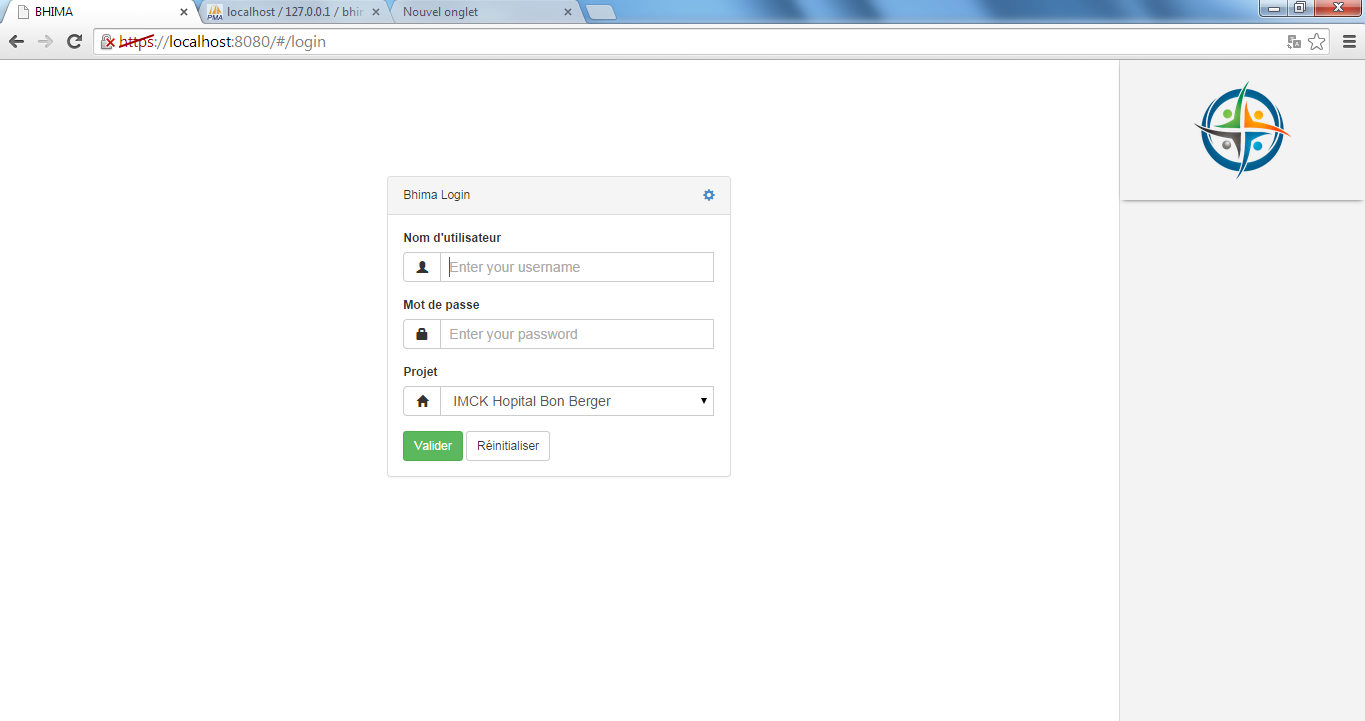
\includegraphics[width=12cm]{pic/login.png}
\end{center}
\caption{Page d'identification et authentification des utilisateurs}
\label{Page d'identification et authentification des utilisateurs}
\end{figure}
\\ L'accès au système n'est garanti que pour ceux qui possèdent un compte utilisateur, si l'utilisateur s'est authentifié alors il sera dirigé vers l'interface principale de l'application qui se présente de la manière suivante.
\newpage
\begin{figure}[h]
\begin{center} 
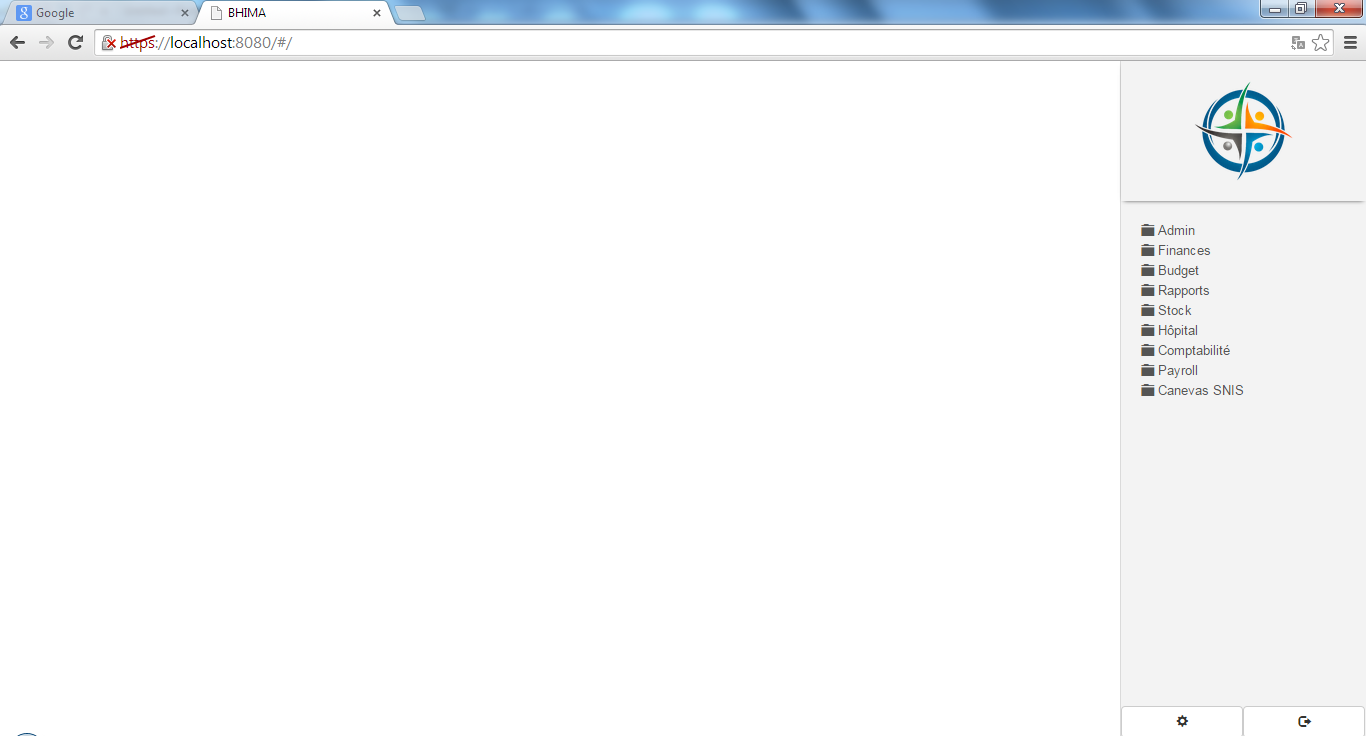
\includegraphics[width=10cm]{pic/mainInterface.png}
\end{center}
\caption{Interface principale de l'application}
\label{Interface principale de l'application}
\end{figure} 
Dans sa partie gauche de la figure ci-dessous on retrouve le logo IMA World Heath Ainsi que l'arborescence qui représente les modules du système auxquels l'utilisateur à accès. En dessous de l'arborescence figure deux boutons, le premier 
\includegraphics[scale=0.5]{pic/lang.png} permet de changer de langue et le second 
\includegraphics[scale=0.5]{pic/logout.png} permet de ce déconnecté du système.

\begin{figure}[h]
\begin{center}
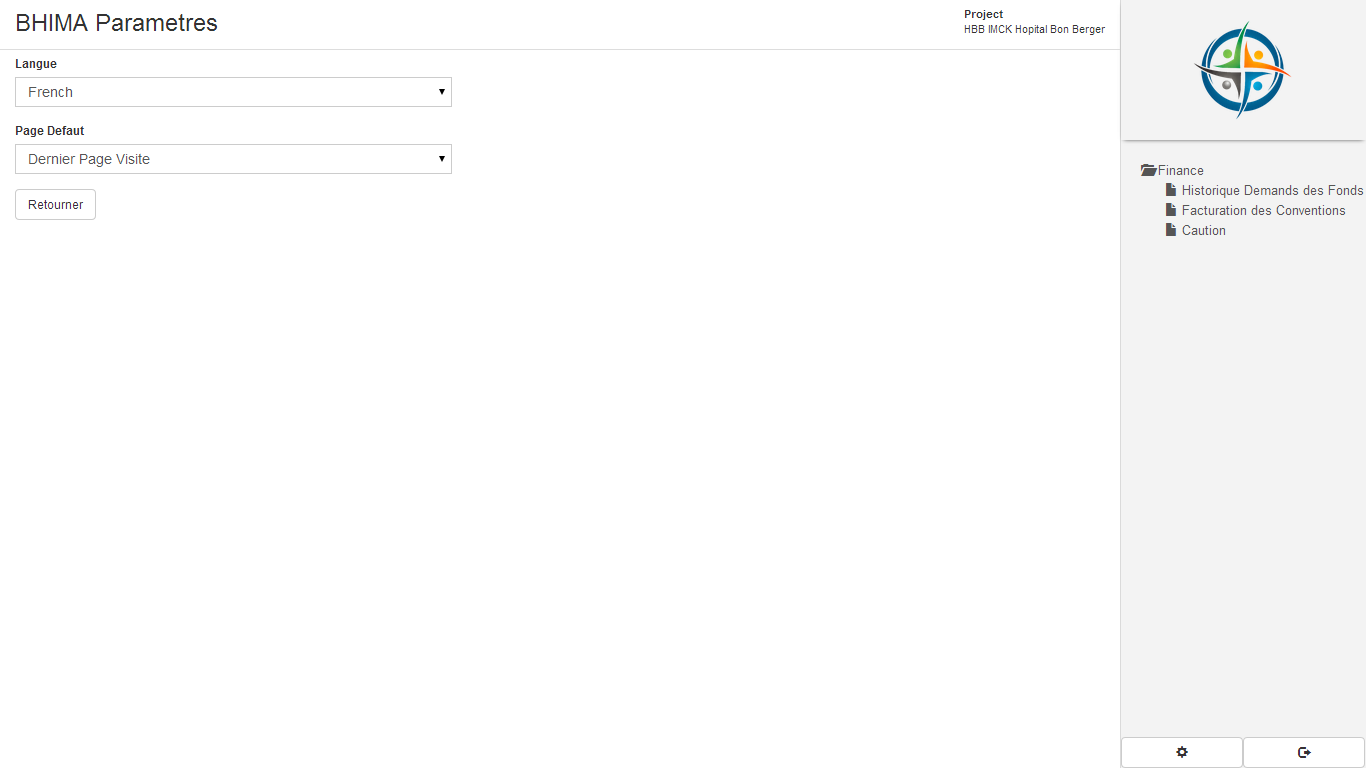
\includegraphics[width=10cm]{pic/changeLang.png}
\end{center}
\caption{Interface principale pour le changement de langue}
\label{Interface principale pour le changement de langue}
\end{figure} 

\section{Utilisation de l'arborescence de navigation}
L'arborescence de navigation contient les liens de chague module de l'application. Les modules sont regroupés en fonction de de leurs fonctionalités dans des dossiers tels que le dossier "Admin" affiché ci-dessous. Dans la première image, le dossier est fermé, en occultant tous les sous modules de ce module. Après le dossier est cliqué, une image d'un dossier ouvert montre que les contenus sont accessibles.

\begin{figure}[h]
\begin{center}
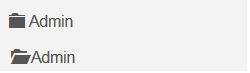
\includegraphics[width=4.5cm]{pic/folder_open_closed.png}
\end{center}
\caption{Etat d'un module ouvert et fermé}
\label{Etat d'un module ouvert et fermé}
\end{figure} 

Cliquant sur le dossier permet d'afficher la liste de sous modules sélectionné par l'utilisateur. Par exemple, ci-dessous, le dossier "Admin" est cliqué dans la premier illustration dans la séconde est ouverte tous ses sous modules.

\begin{figure}[h]
\begin{center}
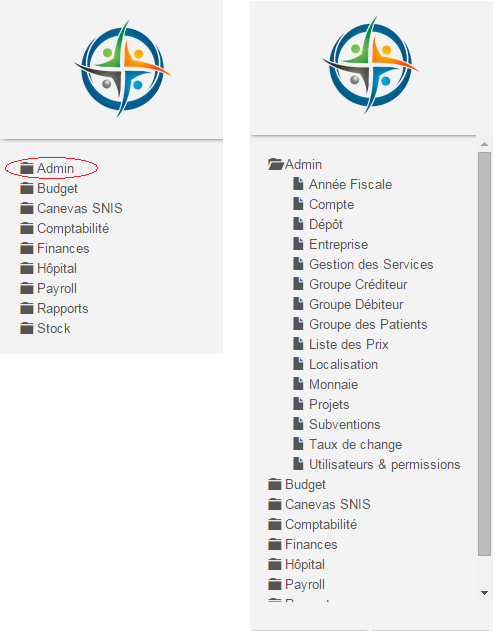
\includegraphics[width=8cm]{pic/open_folder.png}
\end{center}
\caption{Clique sur le dossier "admin" afin de pouvoir visualiser ses sous modules}
\label{Clique sur le dossier "admin" afin de pouvoir visualiser ses sous modules}
\end{figure} 


\newpage
\section{Les modules du système BHIMA}
Le système d'information BHIMA possède plusieurs modules qui sont représenté par l'arborescence ci-dessous.
\begin{figure}[h]
\begin{center}
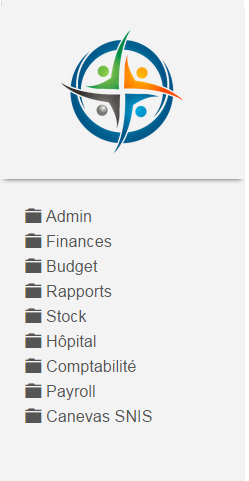
\includegraphics[width=4.5cm]{pic/arbo.png}
\end{center}
\caption{Arborescence du système}
\label{Arborescence du système}
Voici les différentes rubriques qui existent dans le système:
\end{figure} 
% Liste des modules
\begin{itemize}
\item Admin. %•
\item Budget
\item Canevas SNIS
\item Comptabilité
\item Finances
\item Hôpital
\item Payroll
\item Rapports
\item Stock
\end{itemize}


\newpage
%%%%%%%%%%%%%%%%%%%%%%%%%%%%%%%%%%%%%%%%%%%%%
%   MODULES DU SYSTEMES                     %
%%%%%%%%%%%%%%%%%%%%%%%%%%%%%%%%%%%%%%%%%%%%%
    
\chapter{Le module Admin}        
%////////////////////////////////////////////////%
% MODULE ADMIN
Le module admin est composé des sous modules qui permettent d'administrer le système. La figure ci-dessous représente avec exactitude ce module avec ses différents sous éléments.
\begin{figure}[h]
\begin{center}
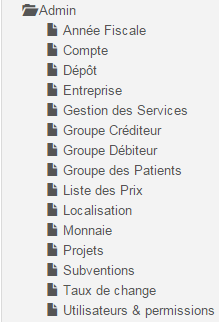
\includegraphics[width=4cm]{pic/s_admin.png}
\end{center}
\caption{Le module Admin et ses sous modules}
\label{Le module Admin et ses sous menus}
\end{figure} 

\newpage
\section{Taux d'échange}
Le module de taux de change, donne la possibilité de définir le taux d'échange du jour. Par souci d'intégrité des données, Le taux d'échange doit être défini chaque jour.


\begin{figure}[h]
\begin{center}
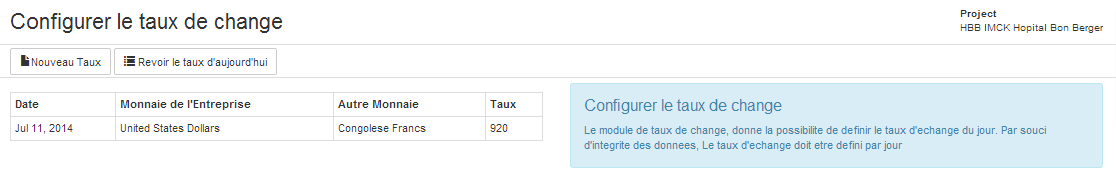
\includegraphics[width=16cm]{pic/FormulaireConfigRate.png}
\end{center}
\caption{Formulaire permettant de configurer le taux de change}
\label{Formulaire permettant de configurer le taux de change}
\end{figure}

\subsection{Nouveau Taux}
Lorsque l'utilisateur click sur le bouton 
\includegraphics[scale=0.7]{pic/NouveauTaux.png}
 Le formulaire ci-après apparait.

\begin{figure}[h]
\begin{center}
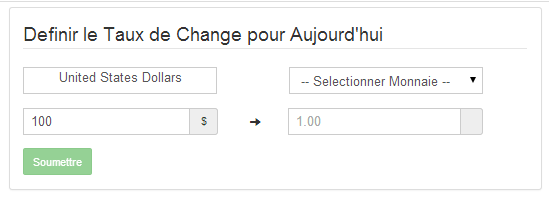
\includegraphics[width=12cm]{pic/DefinirTaux.png}
\end{center}
\caption{Formulaire permettant de definir le taux}
\label{Formulaire permettant de definir le taux}
\end{figure}
\begin{itemize}
\item \textbf{United States Dollars}: est la monnaie principale de l'application, l'équivalence avec d'autres monnaies ne doit se faire qu'avec la somme de 100 Dollars,
\item \textbf{Sélectionner Monnaie}: Affiche la liste des monnaies qui existe dans le système et la zone de saisie qui se retrouve en bas permet de préciser l'équivalence avec la monnaie principale.
\end{itemize}
Après avoir renseigné ce deux champs, un clique sur le bouton \textbf{Soumettre} permet de définir les taux du jour.

\newpage
\subsection{Revoir le taux d'aujourd'hui}
Un clic sur le bouton 
\includegraphics[scale=0.7]{pic/RevoirTaux.png} permet d'afficher toutes les informations sur le taux du jour, comme la montre la figure ci-dessous.
\begin{figure}[h]
\begin{center}
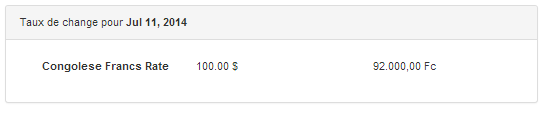
\includegraphics[width=12cm]{pic/ShowRate.png}
\end{center}
\caption{Aperçue du taux du jour}
\label{Aperçue du taux du jour}
\end{figure}
\newpage

\newpage
\chapter{Le module finance}        
%////////////////////////////////////////////////%
Le module finance est composé des sous modules qui permettent d'administrer le finance. La figure ci-dessous représente avec exactitude ce module avec ses différents sous éléments.

\begin{figure}[h]
\begin{center}
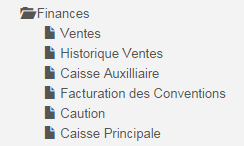
\includegraphics[width=6cm]{pic/FinanceArbo.png}
\end{center}
\caption{Arborescence du module Finance}
\label{Arborescence du module Finance}
\end{figure}



\newpage 
\section{Caisse Principale}
Le module caisse principale, est l'un des principaux modules de cette application, ce module permet d'administrer les recettes ainsi que les dépenses qui s'oppere au sein de l'organisation.

Son interface principale se présente de la manière que voici.

\begin{figure}[h]
\begin{center}
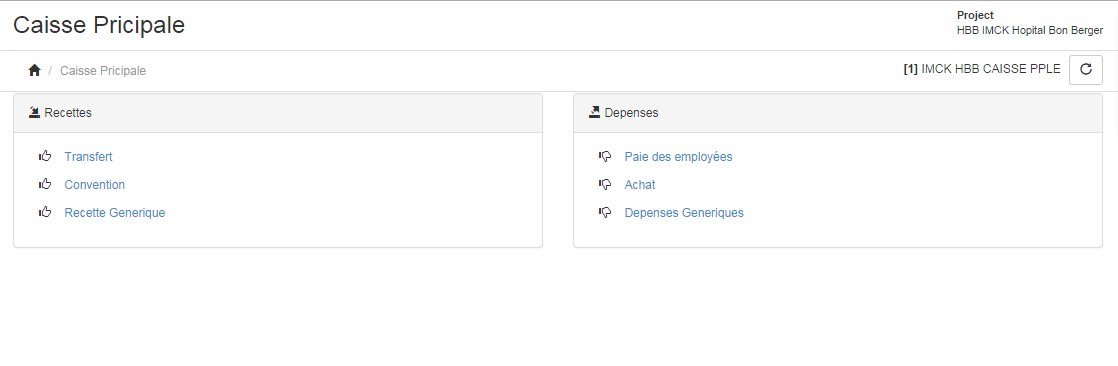
\includegraphics[width=14cm]{pic/caissePrincipale.png}
\end{center}
\caption{Interface principale de la caisse principale}
\label{Interface principale de la caisse principale}
\end{figure}

Cette interface possède deux menus, le premier \textbf{Recettes} et le second \textbf{Dépenses}

\subsection{Recettes : Transfert}
Ce module permet de faire le transfert de fond d'une caisse à une autre, son interface d'utilisation est simple et se présente de la manière suivante.

\begin{figure}[h]
\begin{center}
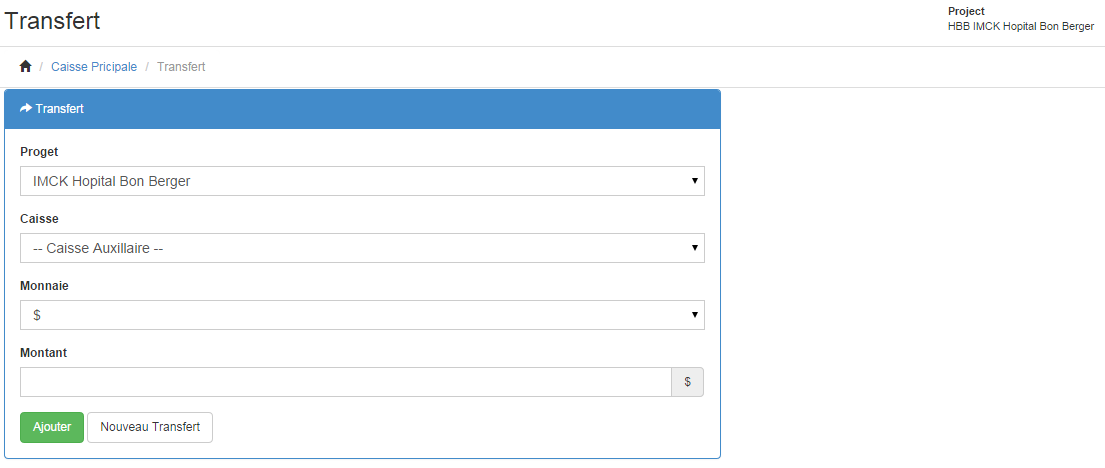
\includegraphics[width=14cm]{pic/Transfert.png}
\end{center}
\caption{Interface principale du module transfert}
\label{Interface principale du module transfert}
\end{figure}

Voici les différents éléments qui composent cet interface.

\begin{itemize}
\item \textbf{Projet}: permet de préciser dans quelle projet s'effectue cet opération. \\
\item \textbf{Caisse}: permet de préciser dans quelle caisse est allouée le fond .\\
\item \textbf{Monnaie}:Pour la monnaie utiliser pour la transaction \\
\item \textbf{Montant}: Pour le motant du transfert\\
\end{itemize}
Après avoir renseigner les différents éléments de ce formulaire, il suffit de cliquer sur le bouton \textbf{Ajouter} pour réaliser le transfert de fond, et pour toute opération de transfert le système générera un reçu.

\newpage
\subsection{Recettes : Convention}
Ce modules permet à des entreprises conventionnées de pouvoir payer les factures de leurs agents ou bien des personnes aux quelles ils prennent en charge, son interface principale se présente de la sorte.

\begin{figure}[h]
\begin{center}
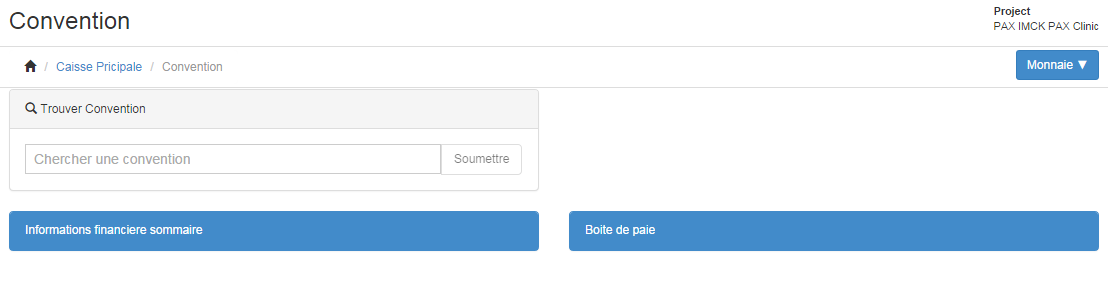
\includegraphics[width=14cm]{pic/conventionMenu.png}
\end{center}
\caption{Interface principale du module Convention}
\label{Interface principale du module Convention}
\end{figure}

Dans le coin superieur gauche il y'a un bouton qui permet de préciser la monnaie qui sera utilisée lors de l'opération du paiement.

En suite il y'a une zone de recherche qui permet de rechercher la convention qui procéder aux paiements, une fois qu'on a retrouver la dite convention, il suffit de cliquer sur le bouton soumettre pour que s'affiche la situation des tous les patients appartenant à la convention ou bien au groupe débiteur choisi, comme le montre la figure ci-après.


\begin{figure}[h]
\begin{center}
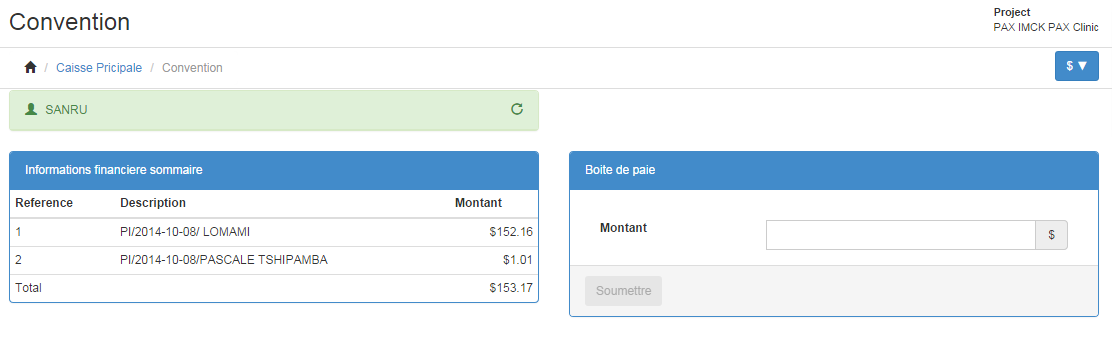
\includegraphics[width=14cm]{pic/conventionMenu2.png}
\end{center}
\caption{Illustration d'un cas de paiement pour un groupe débiteur dont seulement deux patients ont été facturé}
\label{Illustration d'un cas de paiement pour un groupe débiteur dont seulement deux patients ont été facturé}
\end{figure}
 
Dans cette interface nous avons un tableau à gauche qui renseigne sur les informations financières sommaire et en bas du tableau, la totalité de ce que doit le groupe débiteur à l'hôpitale, la zone boite de paiement permet de préciser le montant à payer.

une fois que cette opération est effectué un spéciment de reçu pour les conventions sera généré automatiquement par le système.


\newpage
\subsection{Recettes : Support paiement}
Ce modules permet à des employés ayant prise en charge des patients de pouvoir s'acquiter de leur charges,l'interface principale de ce module se présente de la manière suivante.

\begin{figure}[h]
\begin{center}
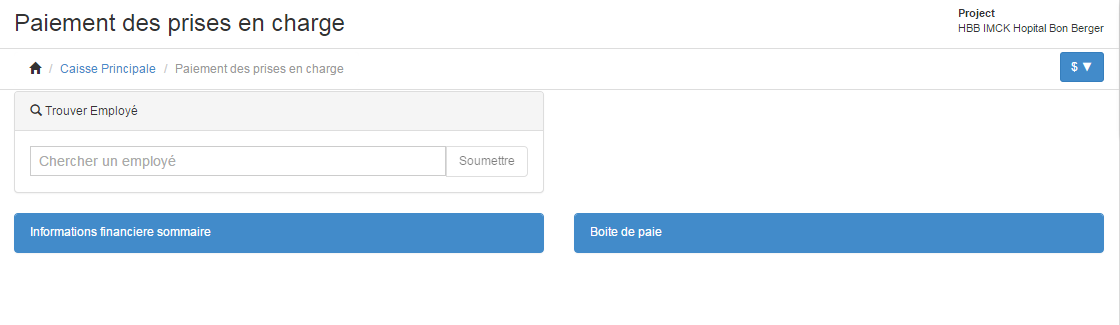
\includegraphics[width=14cm]{pic/InterFacePriseCharge.png}
\end{center}
\caption{Interface principale de paiement de prise en charge}
\label{Interface principale de paiement de prise en charge}
\end{figure}

Dans le coin superieur gauche il y'a un bouton qui permet de préciser la monnaie qui sera utilisée lors de l'opération du paiement.

En suite il y'a une zone de recherche qui permet de rechercher l'employé qui procéde aux paiements, une fois qu'on a retrouver la dite employé, il suffit de cliquer sur le bouton soumettre pour que s'affiche la situation des tous les patients prisent en charge par l'employé, comme le montre la figure ci-après.


\begin{figure}[h]
\begin{center}
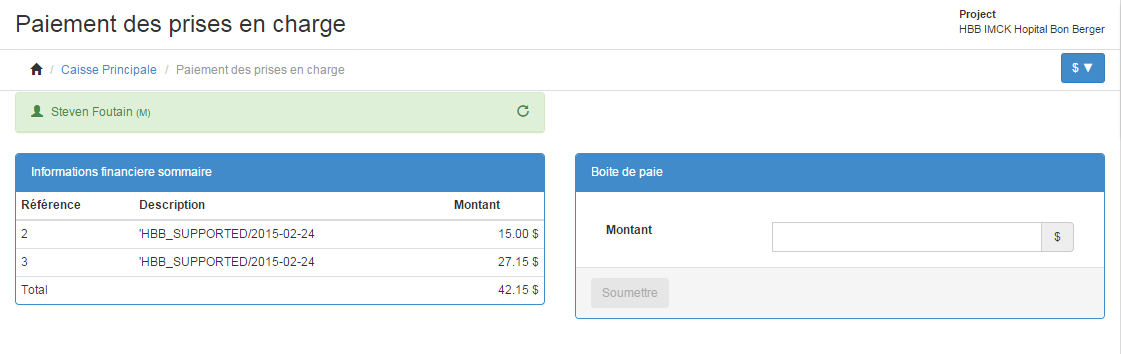
\includegraphics[width=14cm]{pic/PaiemPriseChargeEmploy.png}
\end{center}
\caption{Illustration d'un cas de paiement pour un employé}
\label{Illustration d'un cas de paiement pour un employé}
\end{figure}
 
Dans cette interface nous avons un tableau à gauche qui renseigne sur les informations financières sommaire et en bas du tableau, la totalité de ce que doit le groupe débiteur à l'hôpitale, la zone boite de paiement permet de préciser le montant à payer.

une fois que cette opération est effectué un spéciment de reçu pour les conventions sera généré automatiquement par le système.

\newpage
\subsection{Recettes : Recette Générique}
Les modules recette générique est un module qui a été ajouter au système enfin de pour traquer toutes les recettes générées par l'organisation en dehors des activités liées à l'hôpital, pour l'enregistrement de ce genre des recettes, il faudrait prémierement choisir le compte qui sera utiliser pour l'enregistrement des recettes.

l'interface principale de ce module se présente comme ceci.

\begin{figure}[h]
\begin{center}
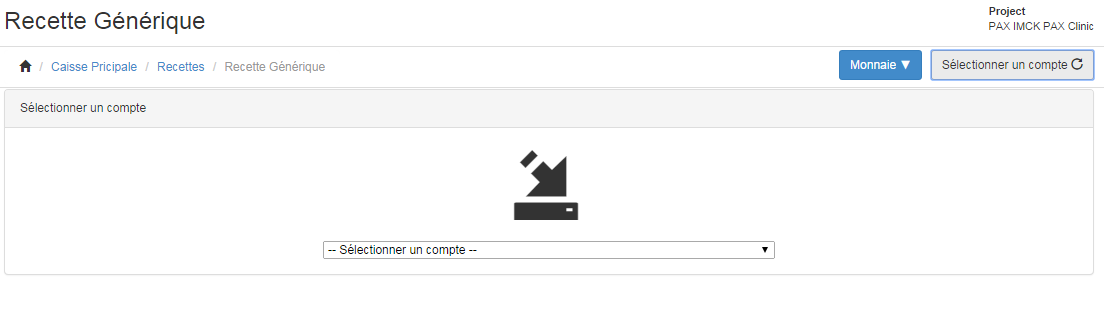
\includegraphics[width=14cm]{pic/recetteGen.png}
\end{center}
\caption{Interface principale permettant de sélectionner un compte}
\label{Interface principale permettant de sélectionner un compte}
\end{figure}

Sur cette interface on aussi un bouton qui permet de préciser la monnaie, et si un compte est déjà choisi par défaut on a la possibilité de la modifier grace au bouton \textbf{Sélectionner un compte}

Après avoir choisi un compte, un deuxième interface apparait, cet interface possède un formulaire qui permet de renseigner les différentes information liée à l'activitité qui a généré une recette telle que la date de la réalisation de la recette, le label ou bien la désignation de la recette, le montant de la recette, il existe aussi un champ \textbf{Référence document ID} qui permet d'attribuer un identifiant unique à l'opération d'enregistrement des recettes.

\begin{figure}[h]
\begin{center}
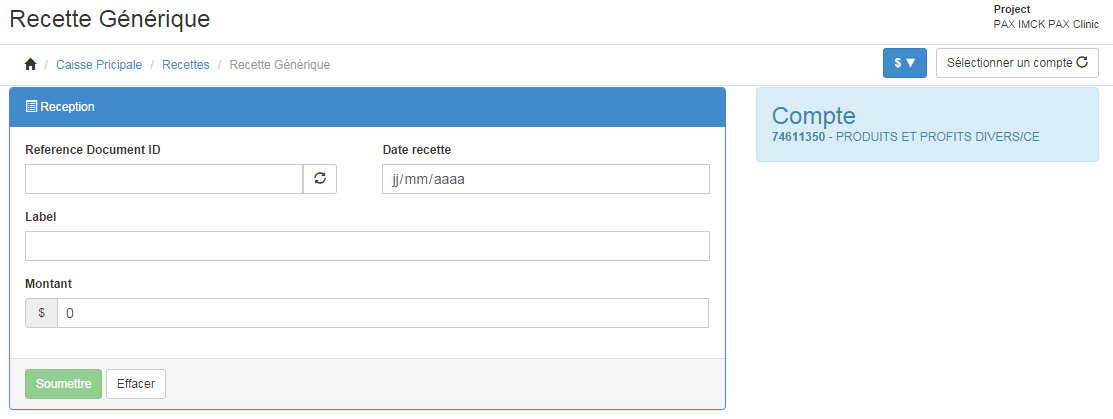
\includegraphics[width=14cm]{pic/recetteGen2.png}
\end{center}
\caption{Interface principale permettant d'enregistrer une recette générique}
\label{Interface principale permettant d'enregistrer une recette générique}
\end{figure}

Dans la zone qui retrouve à droite renseigne sur le compte qui est utilé pour l'opération. Il suffit de cliquer sur le bouton soumettre pour confirmer l'enregistrement d'une recette générique.

\subsection{Dépenses : Paie des employés}
Le module paie des employées permet permet de déterminer les différentes éléments qui seront pris en charge lors du processus de paiement des employés, ce modules est composé d'autre modules qui sont Payroll Multiple, Paiement Taxes et Paiement taxes entreprise. Son interface principale se présente de cette façon.


\begin{figure}[h]
\begin{center}
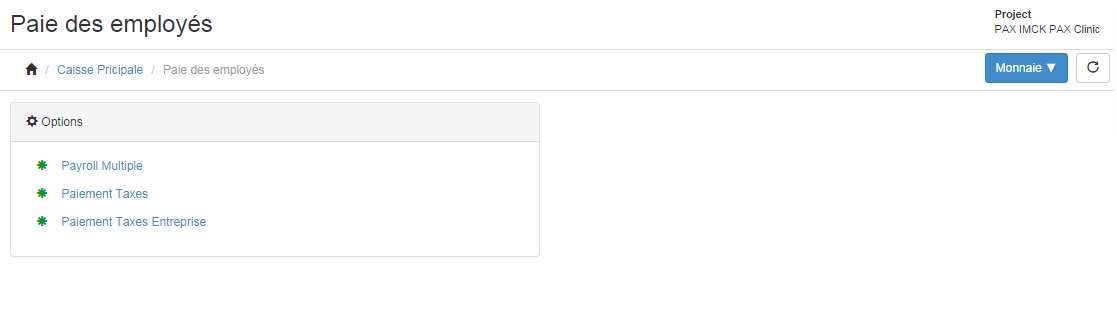
\includegraphics[width=16cm]{pic/paieEmp.png}
\end{center}
\caption{Interface principale du module paie des employés}
\label{Interface principale du module paie des employés}
\end{figure}


\subsection{Dépenses : Paie des employés : Paiement Effectif du Salaire}
Le module paiement des effectifs du salaire n'est utilisable que si il existe une période de paiment pour laquelle ce module n'est pas encore utilisée. ce module dispose ainsi d'une interface principale possédant une liste de choix.

\begin{figure}[h]
\begin{center}
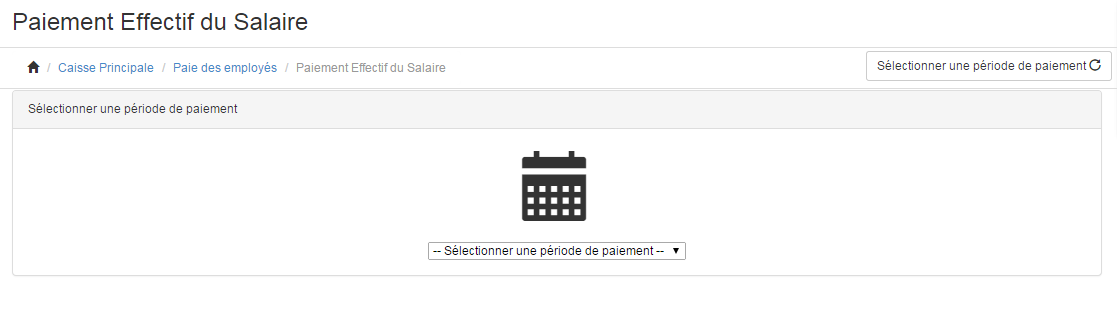
\includegraphics[width=14cm]{pic/selectPeriodPaiSal.png}
\end{center}
\caption{Interface principale permettant de choisir la période de paiement }
\label{Interface principale permettant de choisir la période de paiement }
\end{figure}

Une fois qu'une période de paiement est choisi, l'utilisateur est alors dirigé vers l' interface principale du paiement effectifs des salaires. Cette interface se présente de la manière suivante.

\begin{figure}[h]
\begin{center}
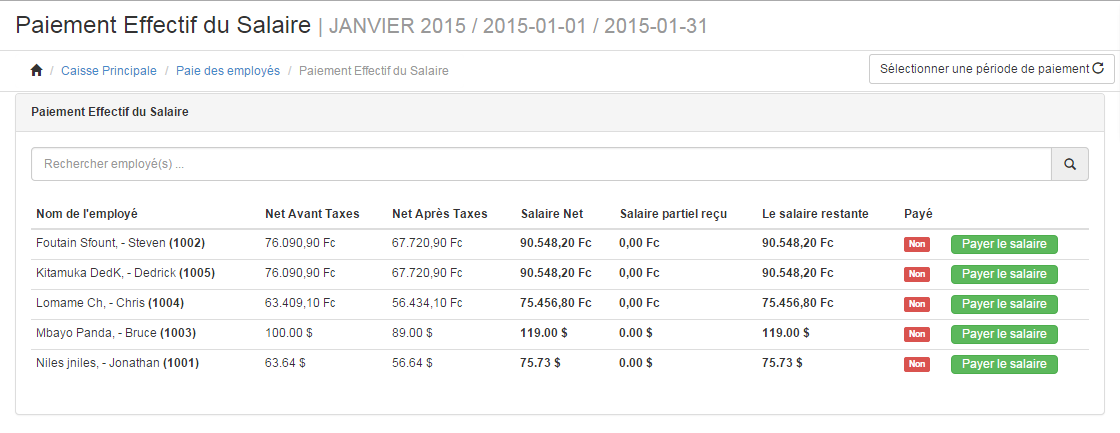
\includegraphics[width=14cm]{pic/paiementSalaire.png}
\end{center}
\caption{Interface principale permettant de confirmer le paiement}
\label{Interface principale permettant de confirmer le paiement}
\end{figure}


Voici les différents éléments de l'interface. Un bouton sélectionner une période de paiement qui permet de revenir vers l'interface permettant de choisir une période de paiement, une barre de recherche permettant de filtrer les différents éléments composant le tableau des employés.

Le tableau est divisé en colonne, il existe les noms des employés, Le net après taxes, le salaire net, le salaire partiel perçu dans le cas où il y'a eu des avances sur salaires, le salaire restante qui est égale au salaire net dans le cas il n'y a pas eu d'avance sur salaire, le status du paiement qui par défaut est 
\includegraphics[scale=0.7]{pic/NonTaxes.png} si l'employé n'est pas encore payée et 
\includegraphics[scale=0.7]{pic/OuiTaxes.png} si elle est payée. pour confirmer le paiement d'un employé, il faudrait cliquer sur le bouton 
\includegraphics[scale=0.7]{pic/PayeSalary.png}

\subsection{Dépenses : Paie des employés : Paiement partiel du salaire}
Le module Paiement partiel du salaire permet de verser à l'employé une partie de son salaire, l'interface principale de ce module se ressemble à celui permettant le paiement effectif à la différence que celui ci permet une redirection vers la page permettant le paiement partiel du salaire.
Le paiement partiel peut se faire en plusieur phase pour vue la somme total perçue ne puissent pas dépasser le salaire net à payer. L'interface d'accueil se présente de la manière suivante.

\begin{figure}[h]
\begin{center}
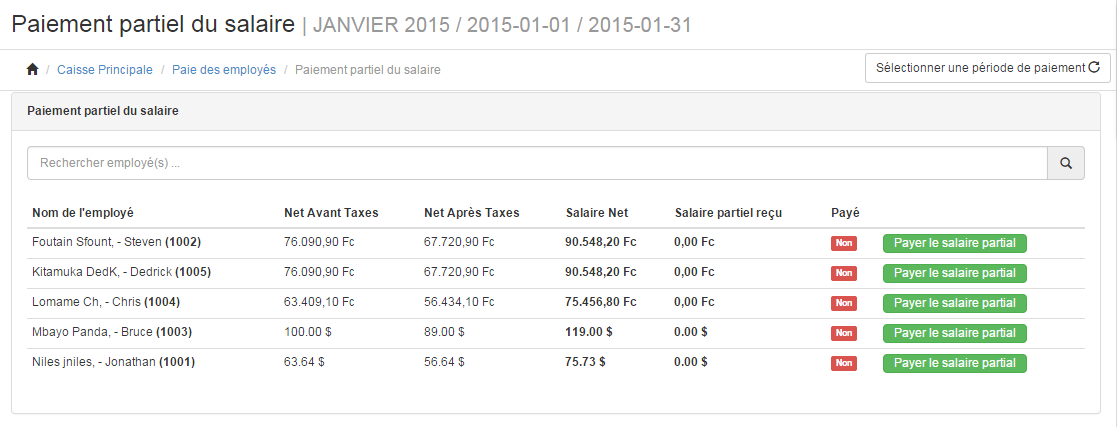
\includegraphics[width=14cm]{pic/PaiePartSalaire.png}
\end{center}
\caption{Interface d'accueil du paiement partiel du salaire}
\label{Interface d'accueil du paiement partiel du salaire}
\end{figure}

Le tableau est divisé en colonne, il existe les noms des employés, Le net après taxes, le salaire net, le salaire partiel perçu dans le cas où il y'a eu des avances sur salaires, le salaire restante, le status du paiement qui par défaut est 
\includegraphics[scale=0.7]{pic/NonTaxes.png} si l'employé n'est pas encore payée et 
\includegraphics[scale=0.7]{pic/OuiTaxes.png} si elle est payée. pour pouvoir procéder au paiement partial du salaire, il suffit de cliquer sur le bouton  
\includegraphics[scale=0.7]{pic/salaryPartial.png} pour visualiser le formulaire du paiement partiel du salaire.

\begin{figure}[h]
\begin{center}
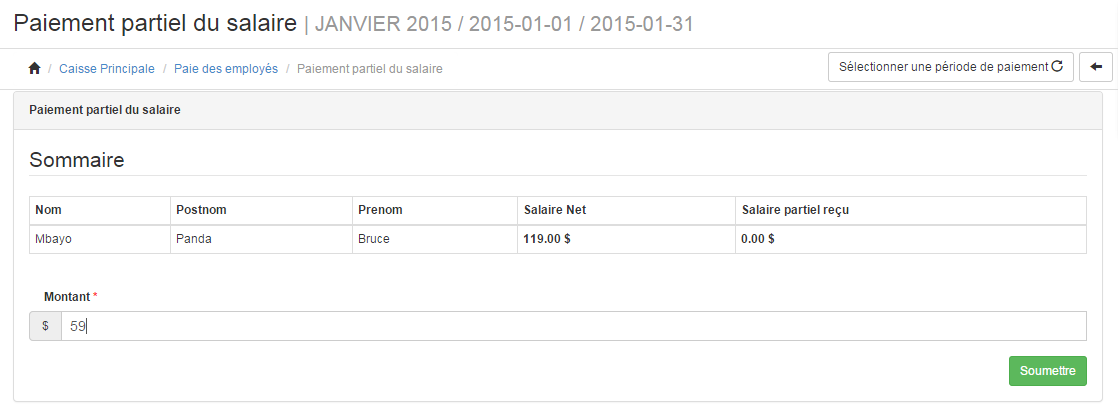
\includegraphics[width=14cm]{pic/FormPartPaiement.png}
\end{center}
\caption{Formulaire permettant le paiement partiel du salaire}
\label{Formulaire permettant le paiement partiel du salaire}
\end{figure}

Dans la figure ci haute on retrouve dans la partie supérieur les éléments sommaires sur le paiement, la zone montant permet de spécifier le montant du paiement partiel qu'on voudrait effectuer et le bouton soumettre permet de declancher le processus.

Si le montant du salaire partiel est supérieur au salaire net ou bien supérieur au salaire restant un message d'alerte s'affiche pour le signaler.

\begin{figure}[h]
\begin{center}

\includegraphics[width=8cm]{pic/errorPartialPaiement.png}
\end{center}
\caption{Message d'erreur en cas de paiement partiel impossible}
\label{Message d'erreur en cas de paiement partiel impossible}
\end{figure}


Les répercutions du paiement partiel du salaire sont visibles dans le module paiement effectif du salaire car le patient ayant bénéficier du salaire partiel du salaire n'obtiendront que leur salaire restant lorsqu'il faudrait procéder au paiement du salaire effectif.

\newpage
\subsection{Dépenses : Paie des employés : Paiement Cotisations}
Le module paiement des cotisations, ce module n'est utilisable que si il existe une période de paiement pour laquelle ce module n'est pas encore utilisé. ce module dispose ainsi d'une interface principale possédant une liste de choix.

\begin{figure}[h]
\begin{center}
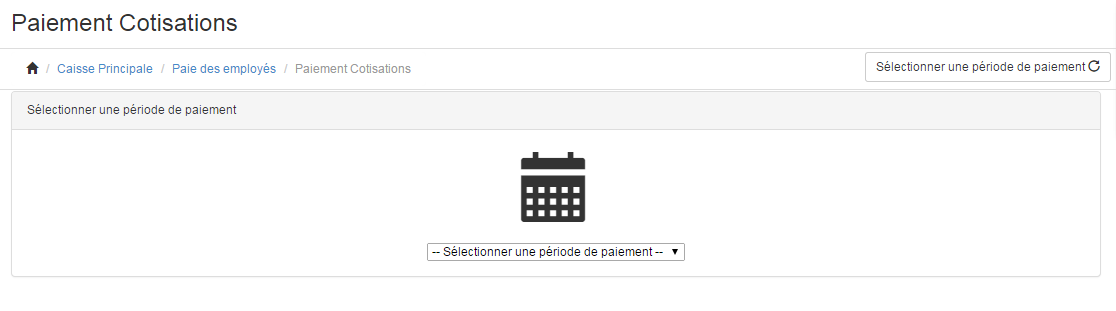
\includegraphics[width=14cm]{pic/paiemCotisations.png}
\end{center}
\caption{Interface principale permettant sélectionner une période de paiement}
\label{Interface principale permettant sélectionner une période de paiement}
\end{figure}

Une fois qu'une période de paiement est choisi, l'utilisateur est alors dirigé vers une interface principale de paiement de des cotisations. Cette interface se présente de la manière suivante.

\begin{figure}[h]
\begin{center}
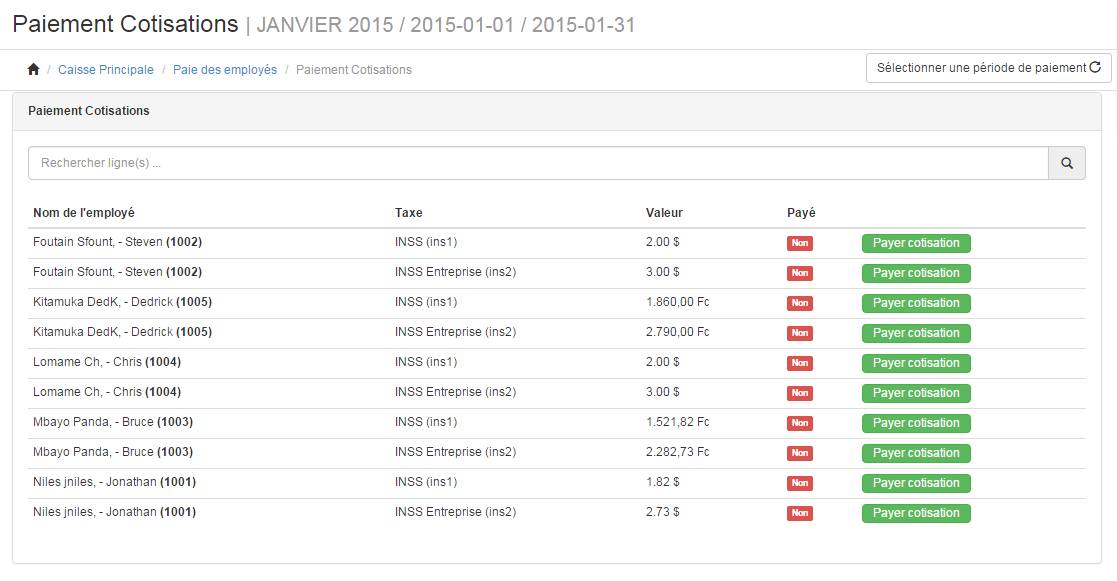
\includegraphics[width=14cm]{pic/PaiemCoInterface.png}
\end{center}
\caption{Interface principale permettant de confirmer le paiement des cotisations}
\label{Interface principale permettant de confirmer le paiement des cotisations}
\end{figure}

Voici les différents éléments de l'interface. Un bouton sélectionner une période de paiement qui permet de revenir vers l'interface permettant de choisir une période de paiement, une barre de recherche permettant de filtrer les différents éléments composant le tableau des employés ainsi que des différentes cotisations.

Le tableau est divisé en colonne, il existe le nom des employés, les différentes types de cotisations, la valeur, le status du paiement qui par défaut est 
\includegraphics[scale=0.7]{pic/NonTaxes.png} si la cotisation n'est pas encore payée et 
\includegraphics[scale=0.7]{pic/OuiTaxes.png} si elle est payée. pour confirmer le paiement d'un cotisation, il faudrait cliquer sur le bouton 
\includegraphics[scale=0.7]{pic/CotPayBouton.png}

\subsection{Dépenses : Paie des employés : Paiement Taxes}
Le module paiement des taxes n'est utilisable que si il existe une période de paiment pour laquelle ce module n'est pas encore utilisé. ce module dispose ainsi d'une interface principale possédant une liste de choix.

\begin{figure}[h]
\begin{center}
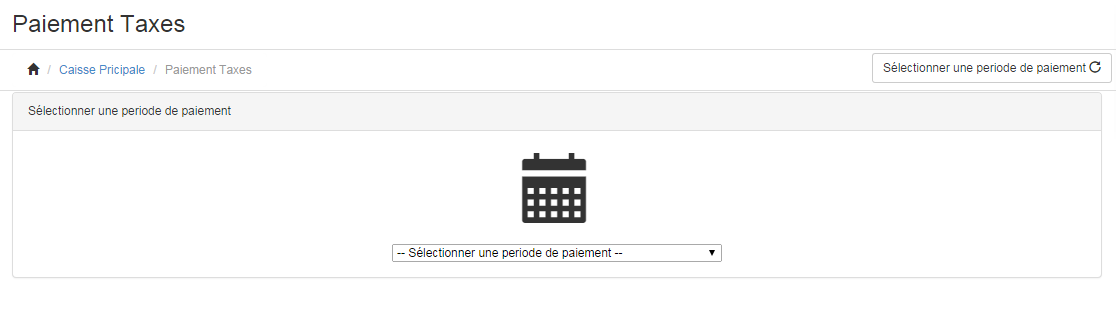
\includegraphics[width=14cm]{pic/PaieTaxes.png}
\end{center}
\caption{Interface principale permettant sélectionner une période de paiement}
\label{Interface principale permettant sélectionner une période de paiement}
\end{figure}

Une fois qu'une période de paiement est choisi, l'utilisateur est alors dirigé vers une interface principale du paiement de taxes. Cette interface se présente de la manière suivante.

\begin{figure}[h]
\begin{center}
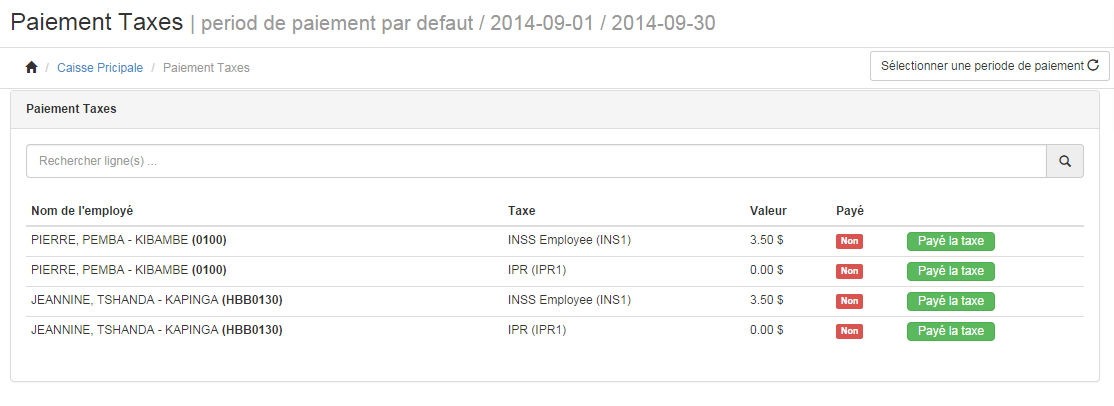
\includegraphics[width=14cm]{pic/PaieTaxes2.png}
\end{center}
\caption{Interface principale permettant de confirmer le paiement}
\label{Interface principale permettant de confirmer le paiement}
\end{figure}


Voici les différents éléments de l'interface. Un bouton sélectionner une période de paiement qui permet de revenir vers l'interface permettant de choisir une période de paiement, une barre de recherche permettant de filtrer les différents éléments composant le tableau des employés ainsi que des différentes taxes.

Le tableau est divisé en colonne, il existe le nom des employés, les types de taxes, la valeur, le status du paiement qui par défaut est 
\includegraphics[scale=0.7]{pic/NonTaxes.png} si la taxe n'est pas encore payée et 
\includegraphics[scale=0.7]{pic/OuiTaxes.png} si elle est payée. pour confirmer le paiement d'une taxe, il faudrait cliquer sur le bouton 
\includegraphics[scale=0.7]{pic/PayeTaxe.png}


\newpage
\subsection{Dépenses : Paie des employés : Paiement Taxes Entreprise}
Le module paiement des taxes Entreprise est similaire à celui permettant le paiement de taxes,  ce module n'est utilisable que si il existe une période de paiement pour laquelle ce module n'est pas encore utilisé. ce module dispose ainsi d'une interface principale possédant une liste de choix.

\begin{figure}[h]
\begin{center}
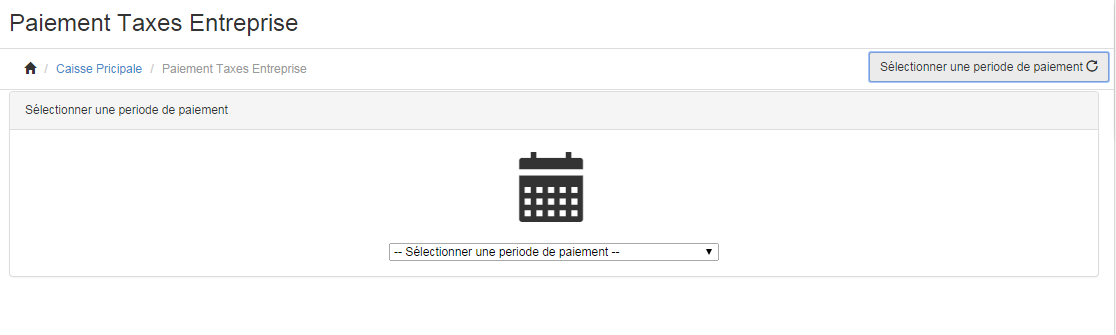
\includegraphics[width=14cm]{pic/PaieTaxesEntre.png}
\end{center}
\caption{Interface principale permettant sélectionner une période de paiement}
\label{Interface principale permettant sélectionner une période de paiement}
\end{figure}

Une fois qu'une période de paiement est choisi, l'utilisateur est alors dirigé vers une interface principale du paiement de taxes de l'entreprise. Cette interface se présente de la manière suivante.

\begin{figure}[h]
\begin{center}
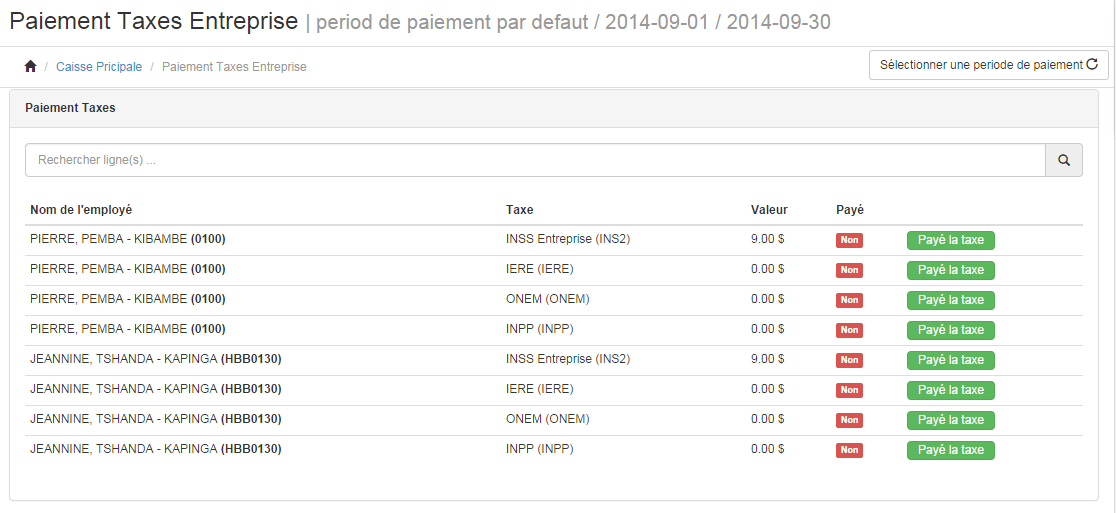
\includegraphics[width=14cm]{pic/PaieTaxesEntre2.png}
\end{center}
\caption{Interface principale permettant de confirmer le paiement}
\label{Interface principale permettant de confirmer le paiement}
\end{figure}


Voici les différents éléments de l'interface. Un bouton sélectionner une période de paiement qui permet de revenir vers l'interface permettant de choisir une période de paiement, une barre de recherche permettant de filtrer les différents éléments composant le tableau des employés ainsi que des différentes taxes.

Le tableau est divisé en colonne, il existe le nom des employés, les types de taxes, la valeur, le status du paiement qui par défaut est 
\includegraphics[scale=0.7]{pic/NonTaxes.png} si la taxe n'est pas encore payée et 
\includegraphics[scale=0.7]{pic/OuiTaxes.png} si elle est payée. pour confirmer le paiement d'une taxe, il faudrait cliquer sur le bouton \includegraphics[scale=0.7]{pic/PayeTaxe.png}

\newpage
\subsection{Dépenses : Achat}
Ce module permet de faire sortir l'argent dans la caisse principale lors qu'une commande d'achat a été établi, voici un apperçu de l'interface du modules Achat.

\begin{figure}[h]
\begin{center}
\includegraphics[width=14cm]{pic/Achat.png}
\end{center}
\caption{Interface principale du module Achat}
\label{Interface principale du module Achat}
\end{figure}

Dans l'interface qui est illustrée, aucun ordre d'achat n'est encore éffectué, mais au cas où il existe des ordres d'achat l'interface se présente de la manière suivante.

\begin{figure}[h]
\begin{center}
\includegraphics[width=14cm]{pic/Achat2.png}
\end{center}
\caption{Module Achat, avec des commandes d'achat}
\label{Module Achat, avec des commandes d'achat}
\end{figure}

On peut remarquer un tableau des différents commandes d'achat qui ne sont pas encore payer, ainsi qu'une permettant de filtrer les commandes d'achat. 

\newpage
Pour que la caisse puisse payer une commande d'achat il faudrait cliquer sur le bouton \includegraphics[scale=0.7]{pic/SelectedPOrder.png} d'une commande d'achat, cet action activera la zone permettant de commencer le processus de paiement, dans cette nouvelle interface on retrouvera les informations rélatives à la commande d'achat, un bouton permettant de confirmer le payement de la commande d'achat ainsi que celui permettant d'annuler une commande d'achat.

\begin{figure}[h]
\begin{center}
\includegraphics[width=14cm]{pic/ConfOrdreAchat.png}
\end{center}
\caption{Illustration de l'interface de confirmation de l'ordre d'achat}
\label{Illustration de l'interface de confirmation de l'ordre d'achat}
\end{figure}

Pour chaque ordre d'achat une preuve de paiement est directement produite par le système.

\begin{figure}[h]
\begin{center}
\includegraphics[width=14cm]{pic/PreuvePaiement.png}
\end{center}
\caption{Apperçue d'un ordre de paiement}
\label{Apperçue d'un ordre de paiement}
\end{figure}

\newpage
\subsection{Recettes : Remboursement}
Ce modules permet à des faires le remboursement aux près des patients mais aussi auprès des employés, ce module permet de régulariser la solde de ces derniers. L'interface principale de ce module se présente de la sorte.

\begin{figure}[h]
\begin{center}
\includegraphics[width=14cm]{pic/remboursementMainInterface.png}
\end{center}
\caption{Interface principale du module Remboursement}
\label{Interface principale du module Remboursement}
\end{figure}

Dans le coin superieur gauche il y'a un bouton qui permet de préciser la monnaie qui sera utilisée lors de l'opération du paiement.

En suite il y'a une zone de recherche qui permet de rechercher  les créditeurs (les employés de l'hôpital) ou bien les débiteurs ( Les patients) pour ce il suffit premièrement de sélectionner la catégorie de la personne qui nécessite un remboursement.


\begin{figure}[h]
\begin{center}
\includegraphics[width=8cm]{pic/SelecCredDeb.png}
\end{center}
\caption{Zone de rechercher des créditeurs ou bien des débiteurs}
\label{Zone de rechercher des créditeurs ou bien des débiteurs}
\end{figure}


une fois que cette opération est effectué on peut rechercher directeur l'indentité de la personne qui necessite un remboursement 

\begin{figure}[h]
\begin{center}
\includegraphics[width=8cm]{pic/RembourDebitor.png}
\end{center}
\caption{Aperçue de la recherche d'un debiteur pour l'opération de remboursement}
\label{Aperçue de la recherche d'un debiteur pour l'opération de remboursement}
\end{figure}



\newpage
\subsection{Dépenses : Dépenses Génériques}
Les modules dépenses génériques permet de tracquer tous les cas des dépenses de fonds au niveau de la caisse principale. l'interface principale de ce module est constituée d'une liste de choix qui permet de préciser le compte concerné par la dépence.
Voici l'illustration de cet interface.

\begin{figure}[h]
\begin{center}
\includegraphics[width=14cm]{pic/DepenseGen.png}
\end{center}
\caption{Apperçue de l'interface principale du module Dépenses Génériques}
\label{Apperçue de l'interface principale du module Dépenses Génériques}
\end{figure}

Sur cette interface on aussi un bouton qui permet de préciser la monnaie, et si un compte est déjà choisi par défaut on a la possibilité de la modifier grace au bouton \textbf{Sélectionner un compte}

\newpage
Après avoir choisi un compte, un deuxième interface apparait, cet interface possède un formulaire qui permet de renseigner les différentes information liée à l'activitité qui a nécéssitée une dépensetelle que la date, le label ou bien la désignation de la dépense, le montant de la dépense, il existe aussi un champ \textbf{Référence document ID} qui permet d'attribuer un identifiant unique à l'opération d'enregistrement des dépenses.

\begin{figure}[h]
\begin{center}
\includegraphics[width=14cm]{pic/recetteGen2.png}
\end{center}
\caption{Interface principale permettant d'enregistrer une recette générique}
\label{Interface principale permettant d'enregistrer une recette générique}
\end{figure}

Dans la zone qui retrouve à droite renseigne sur le compte qui est utilé pour l'opération. Il suffit de cliquer sur le bouton soumettre pour confirmer l'enregistrement de la dépense.

\begin{figure}[h]
\begin{center}
\includegraphics[width=14cm]{pic/FormDepGen.png}
\end{center}
\caption{Apperçue de l'utilisisation du dépense générique}
\label{Apperçue de l'utilisisation du dépense générique}
\end{figure}


\newpage
\chapter{Le module Rapports}        
%////////////////////////////////////////////////%
Le module rapports permet de pouvoir visualiser plusieurs types des rapports résultants du fonctionnements du système, La figure ci-dessous représente avec exactitude ce module avec les différents sous éléments.

\begin{figure}[h]
\begin{center}
\includegraphics[width=4cm]{pic/ArboReport.png}
\end{center}
\caption{Arborescence du module Rapports}
\label{Arborescence du module Rapports}
\end{figure}

\newpage
\section{Plan Comptable}
Le plan comptable permet la visualisation du plan comptable et donne la possibilité de pouvoit imprimer le plan comptable. L'interface principale de ce module se présente de la manière suivante. 

\begin{figure}[h]
\begin{center}
\includegraphics[width=14cm]{pic/PlanComptableAf.png}
\end{center}
\caption{Aperçue du Plan Comptable}
\label{Aperçue du Plan Comptable}
\end{figure}


\newpage
\section{Rapport des Dépenses}
Le rapport des dépenses permet de visualiser toutes les sorties en caisse qui s'éffectue aux niveaux de la caisse principale, l'interface principale de ce module se présente de la manière suivante.

\begin{figure}[h]
\begin{center}
\includegraphics[width=14cm]{pic/RapDepensesInterface.png}
\end{center}
\caption{Interface principale du module Rapport des dépenses}
\label{Interface principale du module Rapport des dépenses}
\end{figure}

La première zone permet de séléctioner une caisse principale par rapport aux monnaies enregistrés, mais aussi de spécifier la date du début et celle de la fin de la recherche. 

Le bouton générer permet l'affichage du tableau du rapport des dépenses. L'interface permettant de visualier le rapport se présente de la manière suivante. Au dessus on retrouve deux boutons. le prémier 
\includegraphics[scale=0.7]{pic/Print.png} permet d'imprimer le rapport et le second \includegraphics[scale=0.7]{pic/refresh.png} permet de faire une nouvelle recherche.

\begin{figure}[h]
\begin{center}
\includegraphics[width=10cm]{pic/RapDepensesApercue.png}
\end{center}
\caption{Aperçue du rapport de dépenses pour une période données}
\label{Aperçue du rapport de dépenses pour une période données}
\end{figure}

Il est aussi possible de pouvoir choisir les depenses respectivement par rapport à la monnaie qui a été utilisé au moment de la transaction.

En bas de page on retrouve les indicateurs permettant de connaitre le nombre des dépenses qui ont été réalisé ainsi que le montant total des recettes ainsi que la possibilité de le visualiser avec différentes monnaies. 

\newpage
\section{Rapport des employés}
Le rapport des Rapport des employés permet de visualiser l'état financier d'un employé. son interface principale se présente de la manière suivante. 

\begin{figure}[h]
\begin{center}
\includegraphics[width=10cm]{pic/EtFinEMp.png}
\end{center}
\caption{Aperçue de l'interface principale de l'état financier d'un employé}
\label{Aperçue de l'interface principale de l'état financier d'un employé}
\end{figure}

Le formulaire possède une zone qui permet la recherche d'un employé dans la liste des employés enregistrés, le bouton générer permet l'affichage du tableau du rapport des employés. L'interface permettant de visualier le rapport se présente de la manière suivante. Au dessus on retrouve deux boutons. le prémier 
\includegraphics[scale=0.7]{pic/Print.png} permet d'imprimer le rapport et le second \includegraphics[scale=0.7]{pic/refresh.png} permet de faire une nouvelle recherche.

Voici un apperçue de la situation financière d'un employé.

\begin{figure}[h]
\begin{center}
\includegraphics[width=14cm]{pic/EtFinancierEmployer.png}
\end{center}
\caption{Aperçue du rapport financier d'un employé}
\label{Aperçue du rapport financier d'un employé}
\end{figure}



%%%%%%%%%%%%%%%%%%%%%%%%%%%%%%%%%%%%%%%%%%%%%%%%%
% Table des matieres
\tableofcontents
\end{document}